\documentclass[conference]{IEEEtran}
\IEEEoverridecommandlockouts
% The preceding line is only needed to identify funding in the first footnote. If that is unneeded, please comment it out.
\usepackage{cite}
\usepackage{amsmath,amssymb,amsfonts}
\usepackage{algorithmic}
\usepackage{graphicx}
\usepackage{textcomp}
\usepackage{xcolor}

% additional packages
\usepackage{bm}
\usepackage{mathtools}
\usepackage{booktabs}
\usepackage{subcaption}

\def\BibTeX{{\rm B\kern-.05em{\sc i\kern-.025em b}\kern-.08em
    T\kern-.1667em\lower.7ex\hbox{E}\kern-.125emX}}
\bibliographystyle{unsrt}

\begin{document}

\title{Weighted Averaging of Multiple Non-collocated Inertial Measurement Units}

\author{\IEEEauthorblockN{1\textsuperscript{st} Yizhou Gao}
% \IEEEauthorblockA{\textit{dept. name of organization (of Aff.)} \\
% \textit{name of organization (of Aff.)}\\
% City, Country \\
% email address or ORCID}
\and
\IEEEauthorblockN{2\textsuperscript{nd} Timothy D. Barfoot}
% \IEEEauthorblockA{\textit{dept. name of organization (of Aff.)} \\
% \textit{name of organization (of Aff.)}\\
% City, Country \\
% email address or ORCID}
}

\maketitle

\begin{abstract}
Multi-IMU fusion has been an effective way of improving MEMS IMU accuracy. In this article, we discuss the averaging technique for multiple IMUs with significant separation. We also present methods of selecting weighting terms such that we either minimize the uncertainty in fused sensor output or arbitrarily placing the reference frame of the combined virtual IMU (VIMU). We tested our method with simulation and evaluated on real dataset. The result shows that the averaging technique works for IMUs with separation and performance gain is observed.
\end{abstract}

\begin{IEEEkeywords}
IMU, multi-IMU, sensor fusion, VINS
\end{IEEEkeywords}

\section{Introduction}

Inertial measurement unit combining a gyroscope and accelerometer that provides measurement of angular velocity and linear acceleration has wide application in robotics and UAS. By integrating the measurement, one can track the relative orientation and position of the system to certain degree of accuracy within reasonable time frame \cite{tang2022_preintegration}. However due to the interoceptive nature of IMU, it is often paired with additional sensors like camera, lidar, or GNSS to reduce drift \cite{alaba2024_gps_and_imu, shan2020_liosam, he2020_visual_imu_and_gps}. In general there are two main approaches to the tracking problem with an IMU - filter-based approach vs. graph optimization approach.

In filter-based approach, IMU measurement is used as process input to an Extended Kalman Filter in propagation step. Then the measurement from other exteroceptive sensors are used for state correction in update step. One such example is MSCKF (Multi-State Constraint Kalman Filter) proposed in \cite{Anastasios2007_MSCKF} which uses IMU for propagation and camera for correction. It proposed a measurement model that directly relate two robot poses based on the landmark observation in camera but independent from the landmark position itself. This allows for efficient tracking without including position of landmarks as part of the state vector as in traditional EKF-SLAM.

For graph optimization approach, such as VINS-MONO \cite{qin2018_vins-mono}, a pose graph is constructed by solving tightly-coupled, nonlinear optimization problem with preintegrated IMU measurement and camera observations. Pose graph optimization is run at the end to ensure global consistency.

Among many sensor configuration with IMU, monocular camera plus IMU is one of the minimal configuration that is well-studied \cite{qin2018_vins-mono, 10616216}. Also IMU has been used heavily as a complimentary sensor for GPS in GNSS-denied environment \cite{1008998, 8987949}. Based on these minimal configurations, various extension has been made. UMS-VINS \cite{jiang2023_UMS-VINS} provides a unified framework for using monocular and stereo cameras in visual-inertial odometry. Also the MSCKF framework \cite{Anastasios2007_MSCKF} also works for multiple cameras with a IMU. There are also works that aim to provide a complete framework to incorporate multiple different sensors in one unified system \cite{10587194}.

Despite works mentioned above, most system and application still only use single IMU in the estimation pipeline. To improve robustness, there have being works in introducing redundant IMUs for fault detection to build fault tolerance system. To detect a measurement error, \cite{Sturza1988_redundant} proposed parity vector based on hypothesis testing. Optimal geometric configuration of multiple redundant IMUs is also explored in \cite{Colomina2004REDUNDANTIF, guerrier2009, xue2023}.

% Further work discuss how to improve the accuracy by fusing multiple low cost IMUs \cite{waegli2008, patel2022_multi-imu, xue2023}.

 In this article the focus is on improving the accuracy of the overall system by leveraging the multiple redundant IMUs onboard in accordance with other sensors provided.

 % As summarized in \cite{patel2022_multi-imu}, for closely place IMUs it is convenient to simply average all IMU measurements after aligning them under a common reference frame.

\section{Related Work}

In this section, we will introduce some prior works on improving the accuracy of multi-IMU system.

% As summarized in \cite{patel2022_multi-imu} there are mainly three ways of

\subsection{Sensor Level Fusion - Virtual IMU}\label{VIMU}

One category of approach is to perform fusion of multiple IMU before using the measurement in inertial navigation system (INS). For example, \cite{jafari2014_PEM} uses Prediction Error Minimization method to model noise of IMUs and use Kalman filter to estimate the optimal process signal. \cite{xue2023} proposed to use Kalman filter to estimate the angular velocity measured by multiple non-orthogonal gyroscopes. Instead of using Kalman filter, an easier approach would be to directly average multiple gyroscopes after aligned under a common virtual IMU frame as discussed in \cite{waegli2008, patel2022_multi-imu, Colomina2004REDUNDANTIF}.

However, averaging of multiple IMUs was not considered due to the additional acceleration terms from rotation (lever arm effect), unless they are closed place and the separation in between is ignored.

\subsection{State Augmentation with Multiple IMUs}\label{augmented}

Typically state estimation problem with single IMU involves tracking the orientation, linear velocity and linear acceleration of the vehicle (commonly defined at the IMU). With additional IMUs, additional state variables like linear acceleration, angular velocity and angular acceleration are added. This allows using the full mechanization model of accelerometer as measurement update in Kalman filter as in \cite{Bancroft2011DataFA, Beaudoin2018_satelite}.

\subsection{Stacked IMU States with Geometric Constraints}\label{constraint}

Another approach is to track individual IMU's state and associate them with geometric constraints \cite{waegli2008, Beaudoin2018_satelite}. Using multiple IMUs and cameras, \cite{Eckenhoff2021_MIMC-VINS} proposed to track all stacked states of base and auxillary IMUs using MSCKF \cite{Anastasios2007_MSCKF}. Assuming the calibrations are known, relative geometric constraints is imposed between states of different IMUs in the form of measurement update in addition to camera observations.

\subsection{Distributed INS}\label{distributed}

Last common approach would be to have individual state estimator for each IMU system each performing local propagation and correction. Simple state fusion is performed with each estimator's estimate \cite{Bancroft2011DataFA, patel2022_multi-imu}.

\subsection{Summary}

As presented, multiple approaches have being proposed. \ref{constraint} would be computationally expensive if number of IMU are large as it has many states all in one Kalman filter. The averaging approach in \ref{VIMU} is the simplest to implement and doesn't significantly alter the existing single IMU framework. Although averaging between accelerometers that are physically separated is not visited due to the lever arm effect, in \ref{methodology} we present that it is still possible to average the accelerometers despite the separation.

\section{Preliminaries}

\subsection{Definitions}

For any quantity $x$ We define $\bar{x} = x + b_x$ as the biased value and $\Tilde{x} = x + n_x$ as the noisy value. If it is both biased and noisy measurement, it is denoted as $y_x$. If a quantity is in the form $x(t)$ then it is a time-varying quantity, otherwise it is time-invariant.

For any point $\textbf{p}$ or vector we define as $\textbf{r}_i^{pi}$ in inertia frame $\mathcal{F}_i$. For example, the vehicle position in inertial frame thus become $\textbf{r}_i^{vi}$.

For rotation matrix or transformation matrix, we have $\textbf{C}_{vi}$ or $\textbf{T}_{vi}$ for transforming point $\textbf{r}_i^{pi}$ expressed in inertial frame $\bm{\mathcal{F}}_i$ into vehicle frame $\bm{\mathcal{F}}_v$ as $\textbf{r}_v^{pv}$.
$$
\left[\begin{matrix} \textbf{r}_v^{pv} \\ 1 \end{matrix}\right]
    = \textbf{T}_{vi} \left[\begin{matrix} \textbf{r}_i^{pi} \\ 1 \end{matrix}\right]
\quad \text{or} \quad
\textbf{r}_v^{pv} = \textbf{C}_{vi} \textbf{r}_i^{pi} + \textbf{r}_v^{iv}
$$

In the rest of the paper, we need to distinguish between body frame and vehicle frame. Body frame $\bm{\mathcal{F}}_b$ is for expressing sensor location relative to some mechanical datum and vehicle frame $\bm{\mathcal{F}}_v$ is for tracking vehicle pose in state estimation pipeline.

When referring the pose of a vehicle, it is a tuple of $\{\textbf{C}_{iv}, \textbf{r}_i^{vi}\}$ which forms the transformation matrix as follow,
$$
\textbf{T}_{iv} = \left[\begin{matrix}
    \textbf{C}_{iv} & \textbf{r}_i^{vi} \\
    \textbf{0} & 1
\end{matrix}\right]
$$

In this document $*^\wedge$ is specifically used for taking a $\mathbb{R}^3$ into skew symmetric matrix. While $*^\wedge$ is used for transforming an element of Lie algebra to corresponding element in Lie group and $*^\vee$ is used for the reverse operation.
$$
\bm{\omega}^\wedge = \left[\begin{matrix}
    0 & -\omega_2 & \omega_1 \\
    \omega_2 & 0 & -\omega_3 \\
    -\omega_1 & \omega_3 & 0
\end{matrix}\right]
$$

\subsection{Rigid-Body Kinematics}

The state propagation using IMU measurement follows the rigid-body kinematics in world fixed frame.
\begin{equation}
\begin{align}
    \dot{\textbf{C}}(t) &= \textbf{C}(t) \bm{\omega}(t)^\wedge \\
    \dot{\textbf{v}}(t) &= \textbf{C}(t) \textbf{a}(t) - \textbf{g} \\
    \dot{\textbf{p}}(t) &= \textbf{v}(t)
\end{align}
\end{equation}

Here $\textbf{C}$ is short for $\textbf{C}_{iv}$, $\textbf{v}$ is short for $\textbf{v}_i^{vi}$, and $\textbf{p}$ is for the position of the vehicle $\textbf{r}_i^{vi}$. These three formed the 9-dof state variables.

In addition, $\textbf{g}$ is the acceleration from gravity and $\bm{\omega}$ and $\textbf{a}$ are the true angular velocity and true linear acceleration in vehicle frame. Thus the goal is to estimate $\bm{\omega}$ and $\textbf{a}$ from measurements of IMUs.

\subsection{IMU Measurement Model}

For the angular velocity measurement from gyroscope we have the following measurement model.

\begin{equation}
    \textbf{y}_\omega(t) = \bm{\omega}(t) + \textbf{b}_\omega(t) + \textbf{n}_\omega(t)
\end{equation}

Where $\textbf{b}_\omega$ is the bias of gyroscope measurement due to random walk and $\textbf{n}_\omega$ is the additive white noise of the measurement. Similarly we have the following measurement model for IMU at vehicle frame. Here $\textbf{b}_a$ is the bias of accelerometer and $\textbf{n}_a$ is the noise of the acceleration measurement.

\begin{equation}
    \textbf{y}_a(t) = \textbf{a}(t) + \textbf{b}_a(t) + \textbf{n}_a(t)
\end{equation}

Bias drifts of IMU are modeled as random walk with the bias drift rate sampled from a Gaussian noise.
\begin{equation}
\begin{split}
    \dot{\textbf{b}}_\omega(t) &= \textbf{w}_\omega(t) \\
    \dot{\textbf{b}}_a(t) &= \textbf{w}_a(t)
\end{split}
\end{equation}

Due to the presence of biases, it is estimated as part of the state vector and subtracted from the raw measurement to get the unbiased measurement for propagation.
\begin{equation}
\begin{split}
    \hat{\bm{\omega}}(t) = \textbf{y}_\omega(t) - \hat{\textbf{b}}_\omega(t) \\
    \hat{\textbf{a}}(t)  = \textbf{y}_a(t) - \hat{\textbf{b}}_a(t)
\end{split}
\end{equation}

For IMU not at vehicle frame, measurement are in each IMU's local frame and we also have additional terms in acceleration measurement due to lever arm effect.
\begin{equation}
    \textbf{y}_{\omega,i}(t) = \textbf{C}_{i}^{-1} \bm{\omega}(t) + \textbf{b}_{\omega, i}(t) + \textbf{n}_{\omega,i}(t)
\end{equation}
\begin{equation}
\begin{split}
    \textbf{y}_{a,i}(t) &= \textbf{C}_i^{-1} \left[ \textbf{a}(t) + \bm{\omega}(t)^\wedge (\bm{\omega}(t)^\wedge \textbf{r}_i) + \bm{\alpha}(t)^\wedge \textbf{r}_i \right] \\
    &+ \textbf{b}_{a,i}(t) + \textbf{n}_{a,i}(t)
\end{split}
\end{equation}

Here we have $\textbf{C}_i$ and $\textbf{r}_i$ short for $\textbf{C}_{vs}$ and $\textbf{r}_v^{sv}$ defining the pose $\textbf{T}_{vs}$ of the $i$-th IMU in vehicle frame (or VIMU frame as oppose to body frame).

\section{Methodology}\label{methodology}

\subsection{Averaging Multiple Gyroscopes}

First we align gyroscope measurements with vehicle frame.
\begin{equation}
    \textbf{C}_{i} \textbf{y}_{\omega,i}(t) = \bm{\omega}(t) + \textbf{C}_{i} \textbf{b}_{\omega, i}(t) + \textbf{C}_{i} \textbf{n}_{\omega,i}(t)
\end{equation}

The weighted average ($\sum_i{a_i} = 1$) of all gyroscope is simply,
\begin{equation}
\begin{split}
    \bar{\textbf{y}}_\omega(t) &= \sum_i{a_i \textbf{C}_{i} \textbf{y}_\omega(t)} \\
    &= \sum_i{a_i \left( \bm{\omega}(t) + \textbf{C}_{i} \textbf{b}_{\omega,i}(t) + \textbf{C}_{i} \textbf{n}_{\omega,i}(t) \right)} \\
    &= \bm{\omega}(t) + \sum_i{a_i \textbf{C}_{i} \textbf{b}_{\omega,i}(t)} + \sum_i{a_i \textbf{C}_{i} \textbf{n}_{\omega,i}(t)}
\end{split}
\end{equation}

We see that the averaged measurement can be summarized as,
\begin{equation}
    \bar{\textbf{y}}_\omega(t) = \bm{\omega}(t) + \bar{\textbf{b}}_\omega(t) + \bar{\textbf{n}}_\omega(t)
\end{equation}

\subsection{Averaging Multiple Accelerometers}

Align the all accelerometer measurements to vehicle frame.
\begin{equation}\label{eqn_accel}
\begin{split}
    \textbf{C}_{i} \textbf{y}_{a,i}(t) &= \textbf{a}(t) + \bm{\omega}(t)^\wedge (\bm{\omega}(t)^\wedge \textbf{r}_i) + \bm{\alpha}(t)^\wedge \textbf{r}_i \\
    &+ \textbf{C}_{i} \textbf{b}_{a,i}(t) + \textbf{C}_{i} \textbf{n}_{a,i}(t)
\end{split}
\end{equation}

Summing equation (\ref{eqn_accel}) of all accelerometer we have,
\begin{equation}
\begin{split}
    \bar{\textbf{y}}_a(t) &= \sum_i{a_i \textbf{C}_{i} \textbf{y}_a(t)} \\
    &= \textbf{a}(t) + \sum_i{a_i \textbf{C}_{i} \textbf{b}_{a,i}(t)} + \sum_i{a_i \textbf{C}_{i} \textbf{n}_{a,i}(t)} \\
    &+ \sum_i{a_i \bm{\omega}(t)^\wedge (\bm{\omega}(t)^\wedge \textbf{r}_i)} + \sum_i{a_i \bm{\alpha}(t)^\wedge \textbf{r}_i} \\
\end{split}
\end{equation}

Using the associate rule $\textbf{a}^\wedge \textbf{b} + \textbf{a}^\wedge \textbf{c} = \textbf{a}^\wedge \left(\textbf{b} + \textbf{c}\right)$, we have,
\begin{equation}
\begin{split}
    \bar{\textbf{y}}_a(t) &= \sum_i{a_i \textbf{C}_{i} \textbf{y}_a(t)} \\
    &= \textbf{a}(t) + \sum_i{a_i \textbf{C}_{i} \textbf{b}_{a,i}(t)} + \sum_i{a_i \textbf{C}_{i} \textbf{n}_{a,i}(t)} \\
    &+ \bm{\omega}(t)^\wedge \left(\bm{\omega}(t)^\wedge \left( \sum_i{a_i \textbf{r}_i} \right) \right) + \bm{\alpha}(t)^\wedge \left( \sum_i{a_i\textbf{r}_i} \right)\\
\end{split}
\end{equation}

If $\sum_i{a_i \textbf{r}_i} = \textbf{0}$ then we can eliminate the last two terms from lever arm effect. This gives,
\begin{equation}
    \bar{\textbf{y}}_a(t) = \textbf{a}(t) + \bar{\textbf{b}}_a(t) + \bar{\textbf{n}}_a(t)
\end{equation}

\subsection{VIMU from Weighted Average}\label{AA}

As we can see, if we choose the vehicle frame and weights of accelerometers such that $\sum_i{a_i \textbf{r}_i} = \textbf{0}$, then we can ignore the separation of all IMUs and fused the accelerometer measurement through averaging.

\textbf{Note that we can choose different weights for averaging gyroscope and accelerometers.}

Since all biases are slow-varying, the combined biases are also slow-varying. So instead of tracking individual biases, only the combined biases are needed. When receiving new set of IMU measurement, we estimate the angular velocity and linear acceleration with the update equations below.
\begin{equation}
\begin{split}
    \hat{\bm{\omega}}(t) = \bar{\textbf{y}}_\omega(t) - \hat{\bar{\textbf{b}}}_\omega(t) \\
    \hat{\textbf{a}}(t)  = \bar{\textbf{y}}_a(t) - \hat{\bar{\textbf{b}}}_a(t)
\end{split}
\end{equation}

The combined measurement is expected to have slower drift and the estimate is expected to be less noisy as well \cite{patel2022_multi-imu}. If having $n$ identical IMUs and equal weight the standard deviation of the combined noise or drift rate is expected to be,
\begin{equation}
    \bar{\sigma} = \frac{\sigma}{\sqrt{n}}
\end{equation}

\subsection{Selecting Weight for Minimal Uncertainty}\label{solve_weight_by_noise}

When selecting weight for gyroscope or for accelerometer when the selection of vehicle frame is flexible, we can minimize the output noise or bias drift rate. Below we take the bias drift as an example but similar idea can be applied to the output noise.

The combined drift rate is as follow. Here we drop the subscript as it is the same for both gyroscope drift and accelerometer drift.
\begin{equation}
    \dot{\bar{\textbf{b}}}(t) = \sum_i{a_i \textbf{C}_i \textbf{w}_i(t)}
\end{equation}

The covariance of the combined drift rate would be the weighted sum of the noise covariance of each IMU.
\begin{equation}
    \bar{\bm{\Sigma}} = \sum_i{a_i^2 \bm{\Sigma}_i}
\end{equation}

One can then solve for the weights that minimize the trace or the sum of the singular value of the covariance.

Since most IMU have isotropic noise for all three axes, the combined variance simplifies to,
\begin{equation}\label{noise_reduction_asym}
    \bar{\sigma}^2 = \sum_i{a_i^2 \sigma_i^2}
\end{equation}

Further more, if using $n$ same IMU and equation weighting, the combined variance is simply,
\begin{equation}\label{noise_reduction_sym}
    \bar{\sigma}^2 = \sum_i{a_i^2 \sigma^2} = n \left(\frac{\sigma}{n}\right)^2 = \frac{\sigma^2}{n}
\end{equation}


\subsection{Selecting Weight for Vehicle Frame Placement}

Given that $\sum_i{a_i \textbf{r}_i} = \textbf{0}$, if there are only two IMUs, we can only place the vehicle frame on the line through the center of the two IMUs. If there are three IMUs, we can only place the vehicle frame on the plane formed by the three IMUs. If there are four non-coplanar IMUs, then in theory, we can place the vehicle frame anywhere. However, placing the vehicle frame outside of the convex hull of the IMUs will increase the output noise which is usually not desired.

When we have a reachable vehicle frame in mind, we need to solve for the weight. Assuming we have arbitrarily many IMUs, then the problem can be formulated as below.
\begin{equation}
\begin{split}
    \min_{w_i}{\frac{1}{2} \sum{w_i^2 \sigma_i^2}} \quad \text{s.t. }
    \begin{cases}
      \sum_i{w_i \textbf{r}_i} &= \textbf{0} \\
      \sum_i{w_i} &= 1
    \end{cases}
\end{split}
\end{equation}

Note that, in this section we will be using $w$ as weight instead of $a$ for convenience. Here $\textbf{r}_i$ is the relative position of the IMUs to the selected vehicle frame. Here we used the objective to reduce output noise as shown in section \ref{solve_weight_by_noise}. Since it is a quadratic programming problem, it is possible to find a close-form solution.

The Lagrangian of the problem is $\mathcal{L} = \frac{1}{2}\textbf{w}^T \bm{\Sigma} \textbf{w} + \bm{\lambda}^T \textbf{R}\textbf{w} + \beta \left( 1 - \textbf{1}^T \textbf{w} \right)$ = 0 where $\bm{\Sigma} = \text{diag}(\sigma_1^2, ..., \sigma_n^2)$, $\textbf{R} = \left[\begin{matrix} \textbf{r}_0 & ... & \textbf{r}_n\end{matrix}\right]$ and $\textbf{1}^T = \left[\begin{matrix}1 & ... & 1\end{matrix}\right]$. This gives the following KKT conditions.
\begin{equation}
\begin{cases}
  \bm{\Sigma}\textbf{w} + \textbf{R}^T \bm{\lambda} - \beta \textbf{1} &= \textbf{0} \\
  \textbf{R} \textbf{w} &= \textbf{0} \\
  \textbf{1}^T \textbf{w} &= 1
\end{cases}
\end{equation}

Left multiple first KKT condition by $\textbf{w}^T$ we have,
\begin{equation}
\textbf{w}^T\bm{\Sigma}\textbf{w} + \textbf{w}^T\textbf{R}\bm{\lambda} - \beta \textbf{w}^T\textbf{1} = 0
\end{equation}

Since $\textbf{w}^T\textbf{R} = \textbf{0}$ and $\textbf{1}\textbf{w} = 1$ we have,
\begin{equation}\label{beta}
    \beta = \textbf{w}^T\bm{\Sigma}\textbf{w}
\end{equation}

Left multiply the first KKT condition by $\bar{\textbf{R}} = \textbf{R}\bm{\Sigma}^{-1}$ gives,
\begin{equation}
\underbrace{\textbf{R}\textbf{w}}_{=\textbf{0}} + \bar{\textbf{R}}\textbf{R}^T\bm{\lambda} - \beta\bar{\textbf{R}}\textbf{1} = 0
\end{equation}

Here we define $\bar{\textbf{r}} = \bar{\textbf{R}}\textbf{1} = \sum{\textbf{r}_i / \sigma_i^2}$ and using pseudo-inverse of $\bar{\textbf{R}}\textbf{R}^T$ we have,

% assuming $\textbf{R}\textbf{R}^T$ is invertible due to having at least 3 non-colocated IMUs then we have,
\begin{equation}\label{lambda}
    \bm{\lambda} = \beta \left(\bar{\textbf{R}}\textbf{R}^T\right)^{+} \textbf{r}
\end{equation}

Substitute equations (\ref{beta}) and (\ref{lambda}) into first KKT condition we have,
\begin{equation}
    \hat{\textbf{w}} = \frac{\textbf{w}}{\textbf{w}^T\bm{\Sigma}\textbf{w}} = \bm{\Sigma}^{-1} \left( \textbf{1} - \textbf{R}^T \left(\bar{\textbf{R}}\textbf{R}^T\right)^{+} \bar{\textbf{r}} \right)
\end{equation}

Lastly since $\sum_i{w_i} = 1$ we need to normalize the intermediate solution to get the final weight for accelerometer.
\begin{equation}
    \textbf{w}^* = \frac{\hat{\textbf{w}}}{\textbf{1}^T \hat{\textbf{w}}}
\end{equation}

\section{Simulation}

\subsection{Data Generation}

First we test our finding in simulation. To generate the simulated data, we first use combination of sinusoidal functions to generate the ground truth angular velocity and linear acceleration in body frame as shown in Figure \ref{fig:omega} and Figure \ref{fig:accel}. Then we integrate it to generate the ground truth trajectory.
% as shown in Figure \ref{fig:trajectory}
For each IMU, we simulate its measurement given the relative transformation in body frame and added noises and biases. Each IMU is sampled at 100 Hz. We selected MPU6050, a common MEMS IMU in the mechatronics community as the example model. All of the above is done using utilities like \texttt{kinematicTrajectory} and \texttt{imuSensor} provided by MATLAB.

We also simulate observations of known landmark from a monocular camera. This turns the estimation problem into a localization problem such that the error is bounded. For each camera frame, we first sample random observations in imaging plane as well as depth (between 2 and 10 m). We then perform reprojection and transform it to inertial frame with the ground truth pose to generate the landmark position. Camera observations arrives at 2 Hz. We selected such a low update rate to allow error to propagate to better show the benefits of averaging.

% \begin{figure*}[ht]
%     \centering
%     \begin{subfigure}[b]{0.4\linewidth}
%         \centering
%         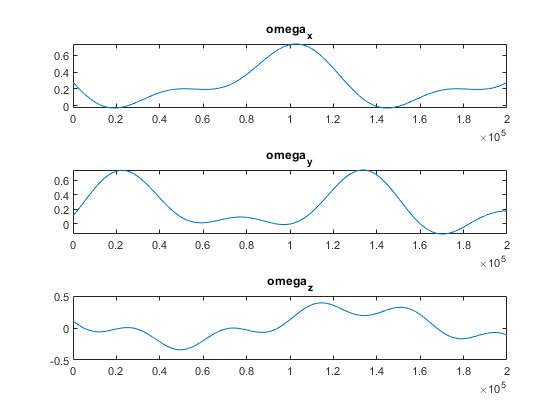
\includegraphics[width=5.8cm]{figures/simulated_omega.png}
%         \caption{Simulated Angular Velocity}
%         \label{fig:omega}
%     \end{subfigure}
%     \begin{subfigure}[b]{0.4\linewidth}
%         \centering
%         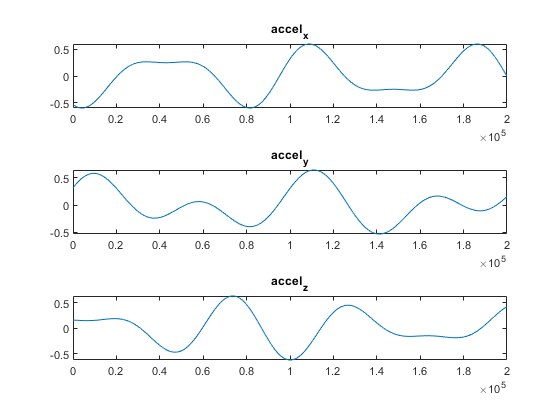
\includegraphics[width=5.8cm]{figures/simulated_accel.png}
%         \caption{Simulated Linear Acceleration}
%         \label{fig:accel}
%     \end{subfigure}
%     \begin{subfigure}[b]{0.4\linewidth}
%         \centering
%         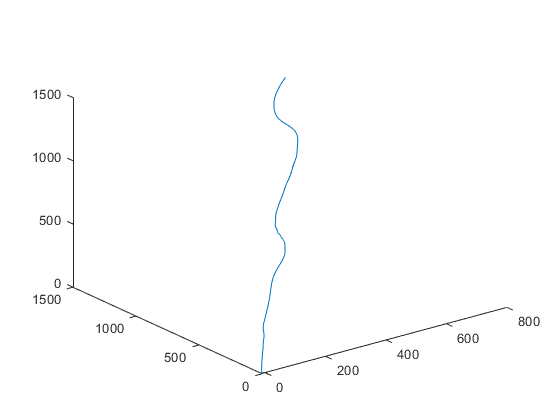
\includegraphics[width=5.8cm]{figures/simulated_trajectory.png}
%         \caption{Ground truth Trajectory from Integration}
%         \label{fig:trajectory}
%     \end{subfigure}
% \caption{Simulated Data Generation with MATLAB}
% \label{fig:switching_diagram}
% \end{figure*}

\begin{figure}
    \centering
    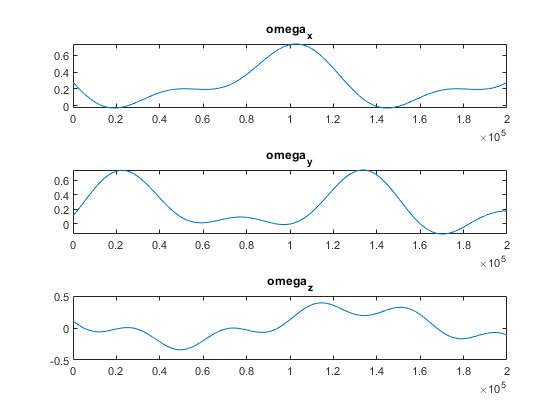
\includegraphics[width=0.85\linewidth]{figures/simulated_omega.png}
    \caption{Simulated Angular Velocity}
    \label{fig:omega}
\end{figure}
\begin{figure}
    \centering
    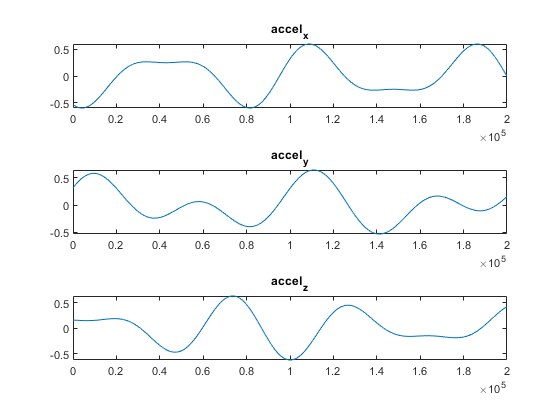
\includegraphics[width=0.85\linewidth]{figures/simulated_accel.png}
    \caption{Simulated Linear Acceleration}
    \label{fig:accel}
\end{figure}
% \begin{figure}
%     \centering
%     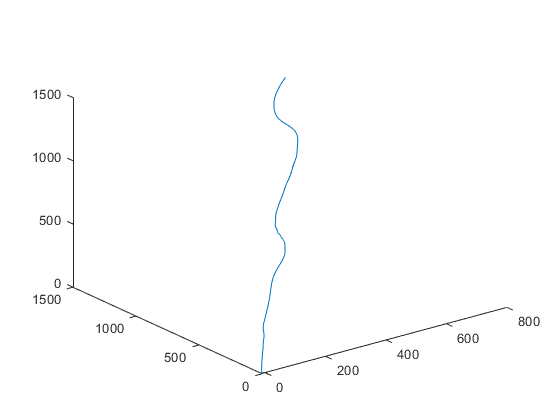
\includegraphics[width=0.85\linewidth]{figures/simulated_trajectory.png}
%     \caption{Ground truth Trajectory from Integration}
%     \label{fig:trajectory}
% \end{figure}

\subsection{Implementation}

For estimator we implemented the \textit{left-}Invariant Extended Kalman Filter (IEKF) \cite{IEKF} as it is more accurate compared to standard EKF methods. At initialization stage, given all IMU poses, we compute the weighting that places the VIMU frame at body frame. Using the weights, we also calculate the combined noises and bias drift rates. When new IMU measurements arrive, they are weighted averaged and then feed into the estimator same as single IMU case. When camera observations arrives, the 2D observations and 3D landmark positions are used for correction step.

\subsection{Experiment Setup}

For performance, we compared results of multiple different IMU configurations summarized in Table \ref{tab:imu_config}. Here symmetric configurations are placing IMUs along the principle axes with an offset of 1 m and random rotation. Assymmetric configurations use IMUs perturbed from symmetric configuration such that different weighting than 1 is required to have VIMU frame at origin of body frame. We place the VIMU frame same as body frame for all configurations for fair comparison of performance. Pose of all IMUs used are summarized in Table \ref{tab:imu_pose}.

\begin{table}[h!]
\centering
\caption{Different IMU Configurations}
\label{tab:imu_config}
\begin{tabular}{cccc}
\toprule
\textbf{Configuration} & \textbf{Category} & \textbf{\# of IMUs} & \textbf{IMU used}  \\
\midrule
IMU-S0 & Baseline  & 1 & 0 \\
\midrule
IMU-S2 & Symmetric & 2 & 1, 2 \\
IMU-S4 & Symmetric & 4 & 1, 2, 3, 4 \\
IMU-S6 & Symmetric & 6 & 1, 2, 3, 4, 5, 6 \\
\midrule
IMU-A2 & Asymmetric & 2 & 11, 12 \\
IMU-A4 & Asymmetric & 4 & 11, 12, 13, 14 \\
IMU-S6 & Asymmetric & 6 & 11, 12, 13, 14, 15, 16 \\

\bottomrule
\end{tabular}
\end{table}

\begin{table}[h!]
\centering
\caption{Pose of IMUs}
\label{tab:imu_pose}
\begin{tabular}{ccc}
\toprule
\textbf{IMU ID} & \textbf{orientation} & \textbf{position} \\
\midrule
0      & $1.000 +0.000i +0.000j + 0.000k$ & [$+0.0, +0.0, +0.0$] \\
\midrule
1      & $0.633 +0.065i -0.025j +0.771k$ & [$+1.0, +0.0, +0.0$] \\
2      & $0.395 +0.795i +0.322j +0.328k$ & [$-1.0, +0.0, +0.0$] \\
3      & $0.533 -0.314i +0.671j +0.409k$ & [$+0.0, +1.0, +0.0$] \\
4      & $0.600 +0.323i +0.620j +0.390k$ & [$+0.0, -1.0, +0.0$] \\
5      & $0.231 +0.495i +0.343j -0.764k$ & [$+0.0, +0.0, +1.0$] \\
6      & $0.744 -0.473i +0.355j +0.310k$ & [$+0.0, +0.0, -1.0$] \\
\midrule
11     & $0.045 -0.112i +0.670j +0.733k$ & [$+0.9, +0.0, +0.0$] \\
12     & $0.223 -0.059i +0.929j -0.289k$ & [$-1.2, +0.0, +0.0$] \\
13     & $0.119 +0.962i +0.245j -0.031k$ & [$+0.3, +1.1, +0.0$] \\
14     & $0.605 +0.708i +0.335j +0.141k$ & [$+0.2, -0.7, +0.0$] \\
15     & $0.004 -0.299i +0.894j +0.333k$ & [$-0.1, +0.2, +1.3$] \\
16     & $0.598 -0.094i -0.669j -0.432k$ & [$+0.4, -0.3, -1.1$] \\
\bottomrule
\end{tabular}
\end{table}

\subsection{Results}

The results are summarized in Table \ref{tab:sim_result}. As more and more IMUs are fused, the mean errors decrease. This matches with the expectation as the combined noises from fused IMU are attenuated as shown by equation \ref{noise_reduction_asym} and \ref{noise_reduction_sym}. Comparing symmetric and asymmetric configuration, the error is marginally larger for asymmetric configuration. This can be explained by the non-uniform weighting which gives higher level of noises than using equal weighting. Overall, the result suggests averaging between IMUs works for both gyroscope and accelerometer measurements disregarding the orientation and separation and the combined measurements are more accurate.

\begin{table}[h!]
\centering
\caption{Simulation Results}
\label{tab:sim_result}
\begin{tabular}{ccccccc}
\toprule
\textbf{Configuration} & \multicolumn{2}{c}{\textbf{Attitude Err (rad)}} & \multicolumn{2}{c}{\textbf{Position Err (m)}} \\
\cmidrule(lr){2-3} \cmidrule(lr){4-5}
& MAE & RMSE & MAE & RMSE \\
\midrule
IMU-S0 & 0.01568 & 0.01873 & 0.11189 & 0.13260 \\
\midrule
IMU-S2 & 0.01278 & 0.01486 & 0.10029 & 0.11540 \\
IMU-S4 & 0.01122 & 0.01319 & 0.09223 & 0.10598 \\
IMU-S6 & 0.01028 & 0.01176 & 0.08950  & 0.10271 \\
\midrule
IMU-A2 & 0.01306 & 0.01514 & 0.10055 & 0.11685 \\
IMU-A4 & 0.01129 & 0.01285 & 0.09222 & 0.10554 \\
IMU-A6 & 0.01083 & 0.01221 & 0.08944 & 0.10077 \\
\bottomrule
\end{tabular}
\end{table}

\section{Real-World Experiment}

For real-world experiment, we choose to perform visual-inertial odometry to understand the performance of averaging in real-life scenario.

\subsection{Dataset}

Most public datasets only contain single IMU. The dataset we find that contains more than one IMU is the PennCOSYVIO dataset \cite{penncosyvio}. This dataset contains three IMUs and multiple cameras. For our experiment, we choose to only use the VI sensor camera as they were provided with complete and correct information regarding intrinsic, extrinsic, and distortion information. We also only used the left camera of the VI sensor such that it forms the minimal configuration with single IMU. This is to not hide the impact of IMUs on performance. We select the VI sensor IMU as the main IMU as it is more accurate compared to the IMUs in the two Tango devices. We will be comparing the performance of using only the VI sensor IMU vs VIMU from averaging all three IMUs.

\subsection{Implementation}

For VIO implementation, we choose to use OpenVINS \cite{openvins} to test the different IMU configurations. OpenVINS is very powerful as it can also estimate camera and IMU intrinsic as well as time offset and extrinsic between IMU and camera. After some tuning, we found that enabling extrinsic and time offset estimation gives the best result over many repeated runs. Also due to the PennCOSYVIO dataset doesn't have a initialization phase when the vehicle is at rest, as a result, we enabled dynamic initialization in OpenVINS.

\subsection{Setup}

To demonstrate the the weighting works as expected, we designed four configuration to test. 1) Single IMU with weight $[\begin{matrix} 1.0 & 0.0 & 0.0 \end{matrix}]$. Here the first weight is for VI sensor IMU, second weight for top Tango IMU, and the third weight is for bottom Tango IMU. 2) Averaged VIMU with weight $[\begin{matrix} 0.33 & 0.33 & 0.33 \end{matrix}]$. 3) VIMU closest to body frame origin with weight $[\begin{matrix} 0.4944 & 0.1546 & 0.3509 \end{matrix}]$. This places the VIMU at $[\begin{matrix} 0.0186 & -0.0012 & -0.0046 \end{matrix}]$ in body frame. 4) We also designed a case when the weight goes negative $[\begin{matrix} 1.2 & -0.1 & -0.1 \end{matrix}]$. This places the VIMU outside of the triangle formed by the three IMUs.

\subsection{Results}

The results are summarized in Table \ref{tab:vio_result}. Example trajectories against ground truth are plotted in \textcolor{red}{Figure} \ref{}.

From the result, different configurations perform similarly. Error reduction from averaging as in simulation is not seen. This is believed to be due to various imperfections from the real-world dataset.

1) Poor calibration. According to the paper of the PennCOSYVIO dataset, the extrinsic calibration is only done between the cameras (for VI sensor only the left camera is calibrated). The IMU positions are assumed from the factory calibration relative to their respective cameras. The chain of transformation can introduces calibration error when averaging the two Tango IMUs with the VI sensor IMU. The VIMU is expected to have less accurate calibration when used with the VI sensor compared to the VI sensor IMU.

2) No static data. Another issue with the dataset is that there is no static stage at the beginning. The initial static stage is crucial for accurate VIO as it allows estimating the initial biases as well as provide known zero initial velocity. As a result, in OpenVINS we have to rely on dynamic initialization which is less accurate compared to static initialization.

3) Vibration and flexing in the fixture. Due to the large separation between all sensors, the physical vibration and deflection in the system can introduce noise and error as well.

It is expected that the noise improvement from averaging is overwhelmed by the imperfection mentioned above. However, from the result we can still conclude that averaging across multiple IMUs with separation does work as expected giving the freedom of placing VIMU frame at preferred location which may previously be not accessible.

\begin{table}[h!]
\centering
\caption{PennCOSYVIO Results}
\label{tab:vio_result}
\begin{tabular}{cccccc}
\toprule
\textbf{Runs} & \textbf{configurations} & \multicolumn{2}{c}{\textbf{Attitude Err (deg)}} & \multicolumn{2}{c}{\textbf{Position Err (m)}} \\
\cmidrule(lr){3-4} \cmidrule(lr){5-6}
 & & MAE & RMSE & MAE & RMSE \\
\midrule
AF & Single   & \textbf{1.335} & \textbf{1.544} & \textbf{0.327} & \textbf{0.409} \\
AF & Averaged & 1.623 & 1.817 & 0.352 & 0.401 \\
AF & Centered & 1.683 & 1.859 & 0.390 & 0.433 \\
AF & Negative & 1.603 & 1.849 & 0.535 & 0.684 \\
\midrule
AS & Single   & \textbf{1.323} & \textbf{1.576} & 0.606 & 0.678 \\
AS & Averaged & 1.709 & 2.103 & 0.585 & 0.667 \\
AS & Centered & 1.390 & 1.696 & 0.479 & 0.533 \\
AS & Negative & 1.425 & 1.619 & \textbf{0.438} & \textbf{0.475} \\
\midrule
BF & Single   & 3.708 & 16.804 & \textbf{0.318} & \textbf{0.369} \\
BF & Averaged & 4.003 & 16.818 & 0.371 & 0.390 \\
BF & Centered & \textbf{3.648} & \textbf{16.789} & 0.366 & 0.402 \\
BF & Negative & 3.723 & 16.822 & 0.887 & 1.279 \\
\midrule
BS & Single   & \textbf{1.416} & \textbf{1.571} & 0.429 & 0.503 \\
BS & Averaged & 1.493 & 1.631 & 0.476 & 0.588 \\
BS & Centered & 1.418 & 1.595 & \textbf{0.318} & \textbf{0.339} \\
BS & Negative & 1.545 & 1.777 & 0.518 & 0.658 \\
\bottomrule
\end{tabular}
\end{table}

\section{Conclusion}

In this paper we presented that in addition to averaging gyroscopes we can also average multiple accelerometers that are physically separated. We also discussed the closed-form solution in determining the weight given design criteria like minimizing noise or placing the VIMU at certain location. Through simulation experiment, we validate the main concept as well as demonstrated the noise reduction benefit of averaging. With real-world dataset, despite the imperfection in the data, we manage to show the averaging technique proposed is a valid approach to take advantage of redundant IMUs on board.

\bibliographystyle{plain}
\bibliography{References.bib}

\end{document}
